\chapter{Métodos e ferramentas}
\label{chap:metodos-ferramentas}

	Neste capítulo é apresentado o método e as ferramentas desenvolvidas e alteradas para
	gerar nossos resultados. O método consiste das seguintes etapas:
	definição da linguagem de programação e das características a serem extraídas;
	códigos-fontes; extração de características; cálculo da matriz de similaridade;
	e projeção e visualização. Em seguida, são especificadas as configurações dessas etapas
	para o contexto do presente trabalho. Por fim, são apresentadas as ferramentas utilizadas para
	extrair as características e visualizar as projeções, bem como as modificações
	necessárias de cada ferramenta.

 	\section{Método}
 	\label{sec:metodo}
 	
	 	Após a revisão da literatura, verificamos que o nosso estudo pode ser dividido
	 	em algumas etapas. Conforme apresentado na \cref{fig:fluxogramaProposta}, primeiro é necessário
	 	escolher qual linguagem de programação será utilizada. Em seguida, deve-se verificar
	 	quais características podem ser extraídas das implementações submetidas utilizando a
	 	linguagem especificada. Posteriormente, é necessário construir a base de dados por
	 	meio da submissão de implementações, realizar a extração de características, minerar
	 	os dados extraídos das submissões e verificar a similaridade entre as implementações.
	 	Por fim, realizar a projeção multidimensional e visualizar os possíveis agrupamentos
	 	formados na projeção.
	 	
	 	\begin{figure}[ht]
	 		\centering
	 		\includegraphics[width=0.75\linewidth]{imagem/fluxogramaProposta}
	 		\caption{Fluxograma das etapas necessárias para a realização do projeto.}
	 		\label{fig:fluxogramaProposta}
	 	\end{figure}
	 	
	 	A \textbf{linguagem de programação} refere-se a definição de qual linguagem será
	 	considerada para as submissões a serem avaliadas. Por exemplo: \texttt{C}, \texttt{Java}
	 	ou \texttt{Python}. Deve ser escolhida conforme a demanda da sua utilização, pela
	 	disponibilidade de cursos de programação ofertado em \acs{MOOC}s ou pelo conhecimento
	 	de ferramentas que possam extrair características de programas escritos nessa linguagem, como o
	 	\texttt{cpplint} para a linguagem \texttt{C}, \texttt{Checkstyle} para
	 	\texttt{Java} e \texttt{pep8} para \texttt{Python}.
	 	
	 	A etapa seguinte trata da \textbf{definição das características a serem extraídas} e será
	 	realizada com base nos trabalhos relacionados (\cref{sec:TrabRel}). Verificamos
	 	que é possível utilizar características originadas de um único tipo de análise
	 	(estática, dinâmica ou do estilo de escrita), bem como associar características
	 	de análises distintas para obter um melhor resultado.
	 	
	 	A etapa \textbf{códigos-fontes} refere-se à construção da base de dados que será
	 	utilizada no estudo. Tal base tem que possuir uma quantidade considerável de
	 	submissões de códigos-fontes, devido a quantidade de usuários que utilizam o \acs{MOOC},
	 	para que seja possível avaliar o desenvolvimento do projeto com uma quantidade
	 	condizente com o número de usuários.
	 	
	 	A \textbf{extração de características} é a fase na qual escolhe-se uma ferramenta
	 	disponibilizada livremente pela Internet que extraia as características selecionadas
	 	previamente, visto que não desejamos criar uma ferramenta para esse fim. Tal estágio
	 	é responsável pela adaptação das ferramentas selecionadas anteriormente para que seja
	 	possível obter as características e salvá-las em algum tipo de arquivo, como o
	 	formato \texttt{XML} e o \texttt{CSV}, por exemplo.
	 	
	 	Na etapa de \textbf{cálculo da matriz de similaridade} analisam-se os dados obtidos a
	 	fim de verificar a similaridade entre as diferentes instâncias de submissões com relação
	 	às características extraídas. Isso permite a utilização de técnicas para verificar a similaridade
	 	entre os códigos-fontes, como a similaridade do cosseno.
	 	
	 	Por fim, \textbf{projeção e visualização} refere-se ao emprego de técnicas de
	 	projeção multidimensional para que seja possível realizar um mapeamento de um
	 	espaço multidimensional (alta dimensionalidade) para um espaço de baixa
	 	dimensionalidade (bidimensional ou tridimensional), buscando a menor perda de
	 	informação possível, como a manutenção das relações de similaridade do espaço
	 	multidimensional no espaço de baixa dimensionalidade. Neste estudo uma dimensão
	 	é referente a uma característica extraída da implementação. Portanto, a quantidade
	 	de dimensões nos dados é igual a quantidade de características extraídas. Com isso,
	 	é necessário selecionar uma técnica para diminuir um espaço n-dimensional para
	 	duas ou três dimensões a fim de realizar a visualização exploratória para
	 	identificar padrões nos dados e possíveis agrupamentos formados.
	 	
	 	No caso das características extraídas não serem relevantes o suficiente, a
	 	visualização não será capaz de produzir modelos gráficos significativos que
	 	evidenciem os padrões existentes nos dados, sendo necessário voltar à segunda
	 	etapa para definição de outras características a serem extraídas.
	 	
	 	Nosso objetivo, por meio dessas etapas, consistiu no desenvolvimento de subsídios
	 	para avaliação de programas, utilizando técnicas de visualização para auxiliar os professores a
	 	corrigirem todas as submissões, considerando o tempo de correção e a qualidade do
	 	\foreign{feedback} referente a \foreign{ScienceView} para o professor.
	 	Por isso, temos duas questões de pesquisa (QP):
	 	
	 	\begin{itemize}
	 		\item \textbf{QP$_1$}: o algoritmo de agrupamento produz grupos de códigos-fontes
	 		com boa qualidade?
	 		\item \textbf{QP$_2$}: a utilização de subsídios de avaliação reduz o tempo
	 		de correção de todas as submissões?
	 	\end{itemize}
	 	
	 	O subsídio de avaliação foi uma adaptação da ferramenta \texttt{ScienceView}
	 	\cite{Alencar-etal:2012} que, originalmente, verifica as mudanças nas relações
	 	de artigos científicos com o decorrer do tempo, utilizando técnicas de mineração
	 	visual embasadas em uma técnica de projeção multidimensional chamada \acl{T-LSP}
	 	\cite{Alencar}.
	 	
	 	Para validar o tempo gasto para todas as correções, foram criado dois grupos de
	 	professores. Um grupo utilizou a técnica proposta nessa pesquisa para realizar
	 	a avaliação das implementações, enquanto o outro grupo avaliou as mesmas submissões
	 	manualmente. Além disso, avaliamos o \foreign{feedback} da ferramenta para os
	 	professores por meio de \foreign{survey} e questionário para cada professor.
	 		
	\section{Considerações para avaliações}

		Considerando os estágios estabelecidos no método descrito na Seção anterior
		(\ref{fig:fluxogramaProposta}), foram definidos requisitos e elementos a serem
		empregados na avaliação dos códigos-fontes neste trabalho, apresentados
		nas seções seguintes.

		\subsection{Definição da linguagem de programação}
		
			% TODO: inversão dos argumentos
			Foi definido a utilização da linguagem de programação Python. A escolha foi
			devido a disponibilidade de cursos sobre introdução a programação utilizando
			\texttt{Python} em diversos \acs{MOOC}s e cursos de graduação. Como também
			o conhecimento prévio de ferramentas que possam auxiliar na verificação
			e extração de características.

		\subsection{Definição das características a serem extraídas}

			Com base em todos os trabalhos relacionados, podemos perceber que os três
			tipos de análise -- estática, estilo de escrita e dinâmica -- obtiveram
			bons resultados. Isso nos possibilitou decidir qual tipo de análise
			utilizar. Desta forma, optamos pelo tipo de análise por meio da disponibilidade
			de ferramentas para verificar tais tipos de características e que possuíssem
			código aberto para realizar adaptações a fim de alcançar nosso objetivo.
			Desde que posteriormente ocorra uma seleção das características mais relevantes
			para avaliação, a escolha natural das características, apresentadas a seguir,
			não	afeta a qualidade das projeções.A seleção de características relevantes
			faz parte dos trabalhos futuros.

			Considerando a combinação de características originadas de tipos de análises
			distintas, utilizamos uma combinação de aspectos provenientes da análise  
			estática e do estilo de escrita. A escolha da análise estática deu-se pela
			possibilidade de implementações para solucionar o mesmo problema possuírem
			o mesmo tamanho. Adicionalmente, a organização do código, realizado pelo programador,
			pode impactar no entendimento da solução do problema: por isso a escolha da
			análise do estilo de escrita.  Não utilizaremos a análise dinâmica pela falta
			de conhecimento de ferramentas que nos forneça tal característica e pelo pouco
			tempo hábil para implementação de uma ferramenta para realizar esse tipo de
			análise e validação dessa ferramenta.
			
			As características a serem extraídas da análise estática foram a quantidade
			de linhas de código e a complexidade ciclomática da implementação. Em relação
			a análise do estilo de escrita, foram consideradas todas as violações do estilo de
			escrita definido pelo \texttt{PEP 8}~\cite{van2001pep}. 

		\subsection{Códigos-fontes}	
		
			Essa etapa refere-se a construção da base de dados que será utilizada no experimento.
			É necessário que o conjunto de implementações obtenha uma quantidade considerável de
			códigos-fontes a fim de avaliar a utilização da ferramenta para \acs{MOOC}. A
			base de dados desse estudo possui somente implementações desenvolvidas em \texttt{Python}
			de um curso introdutório à Computação e Programação.
			
		\subsection{Extração de características}
					
			Obtivemos as informações necessárias por meio da análise estática e do estilo de   
			escrita com o auxílio das ferramentas \texttt{pep8} \cite{pep8} e \texttt{mccabe}
			\cite{mccabe} que funcionam como \foreign{plugins} para o \texttt{flake8}.
			Extraímos da análise estática, além do estilo de escrita, a quantidade de linhas
			do código-fonte e a complexidade ciclomática de cada \foreign{plugin}, respectivamente.
			Contudo, o foco do \texttt{pep8} é verificar se o estilo de escrita PEP 8 \cite{van2001pep}
			está sendo praticado corretamente. Por esse motivo, extraímos as características
			relacionadas a: indentação (\cref{tab:pep8E100}); espaços em branco
			(\cref{tab:pep8E200}); linhas em branco (\cref{tab:pep8E300}); declaração de
			importação de bibliotecas (\cref{tab:pep8E400}); tamanho da linha (\cref{tab:pep8E500});
			quantidade de instruções por linha e formas de instrução (\cref{tab:pep8E700}); por fim,
			verificação de sintaxe e geração de \foreign{tokens} (\cref{tab:pep8E900}). Todas essas
			tabelas estão presentes no \cref{apendice:pep8}.
		
%	A indentação possui as seguintes características: tabulações e espaços misturados;
%	o nível não possui indentação, mas foi encontrado espaços em branco ou uma indentação,
%	ambas podendo ser seguida de um comentário; o nível possui uma indentação, entretanto,
%	esse não foi encontrado ou foi encontrado seguido de um comentário; há espaços, contudo
%	é menor que uma tabulação de 4 espaços, definido como padrão no \texttt{PEP8}; e em
%	instruções de múltiplas linhas verifica se as linhas seguintes estão indentadas com
%	a primeira linha da instrução.
%	
%	Os espaços em branco são analisados em chamadas de função, atribuições, operações
%	lógicas e aritméticas, entre palavras reservadas e comentário. Em chamadas de
%	funções constata a presença ou falta de espaço em branco depois dos \foreign{tokens}
%	\texttt{(}, \texttt{\{} e \texttt{[} ou antes dos \foreign{tokens} \texttt{)},
%	\texttt{\}}, \texttt{]}, como também antes de \texttt{(} e \texttt{[} no caso de
%	querer acessar um índice de uma lista, por exemplo. Nas atribuições compreende se
%	não há espaço em branco entre o operador de atribuição, enquanto nas operações
%	lógicas e aritméticas constata se não há espaço entre seus operadores.
%	
%	% linhas em branco entre métodos e, entre declaração da classe e um método da classe
%	A verificação de linhas em brancos é utilizada para observar como um método está
%	separado de outro método, bem como da declaração da classe. Os métodos devem estar
%	separados por duas linhas em branco, enquanto a declaração da classe e o primeiro
%	método deve estar separado por apenas uma linha em branco. Caso essas duas
%	características não sejam cumpridas, além de possuir várias linhas em branco,
%	o analisador gera um erro.
%	
%	% importação de bibliotecas
%	A quantidade de bibliotecas que estão sendo importadas também é observado. O
%	\texttt{PEP8} considera importar apenas uma biblioteca por linha. Portanto,
%	o \foreign{plugin}, irá detectar a importação de duas ou mais bibliotecas na
%	mesma linha.
%	
%	% tamanho da linha
%	O analisador também verifica o tamanho, em caracteres, de uma linha. Uma mensagem
%	de erro ocorre quando a linha possuir 80 caracteres ou mais. Além disso, é
%	contraindicado utilizar uma barra invertida seguido de uma nova linha quando estiver
%	entre colchetes ou parenteses.
%	
%	% quantidade de instruções por linha e formas de instrução
%	A quantidade de instruções por linha menciona as instruções que podem ser separadas
%	por \texttt{:} (dois-pontos) ou \texttt{;} (ponto e vírgula). O primeiro caso pode
%	ocorrer em uma declaração de condicional e sua primeira instrução. Enquanto, o segundo
%	caso, ocorre entre duas instruções. Por fim, as formas de instruções verifica: se uma
%	instrução é terminada com \texttt{;}; utilização de operadores lógicos para comparar
%	valores únicos (\foreign{singletons}), ao invés de utilizar \texttt{is} ou \texttt{is not};
%	a utilização de \texttt{not in} para verificar se uma variável está contida em outra e
%	\texttt{is not} para comparar objetos; por fim, a comparação de tipos é realizado pelo
%	\texttt{isinstance()}.
%	
%	% verificação de sintaxe e geração de tokens
%	Por fim, o \texttt{PEP8} também verifica se a sintaxe do código-fonte é valida.
%	\textbf{Falta falar sobre o erro E902, mas não entendi a definição no PEP8:
%		"Tokenize the file, run physical line checks and yield tokens."}
	
			A ferramenta \texttt{mccabe} \cite{mccabe2013} fornece informações sobre a
			complexidade ciclomática \cite{mccabe} de cada função ou método implementado.
			Essa complexidade é referente às estruturas de decisões implementadas \cite{mccabe},
			ou seja, seu cálculo é realizado com base na utilização de \texttt{if/else} e laços
			de repetição.
			
		
		\subsection{Cálculo da matriz de similaridade}
		
			Com a finalidade de encontrar relações de similaridade entre os códigos-fontes
			com base nos valores das características extraídas para eles, utilizamos a
			técnica de similaridade do cosseno. Visto que, durante a extração de
			características obtemos uma representação matricial dos dados. Essa matriz é
			tipicamente esparsa -- possui grande quantidade de 0 (zeros). 
			A ocorrência da grande quantidade de 0 (zeros) ocorre pela busca
			dos programadores em implementar suas soluções computacionais corretamente.
%			Nesse tipo de situação, a similaridade do cosseno é conhecida por apresentar
%			bons resultados.
			% TODO: Igor pediu referência da afirmação anterior. Reformulei para a frase abaixo
			Nesse tipo de situação, a similaridade do cosseno é mais utilizada por não
			favorecer comparações entre 0 (zeros)~\cite{Alencar}.
			Por isso, ela faz com que implementações para problemas distintos não sejam
			consideradas semelhantes devido a quantidade de 0 (zeros) nas mesmas
			características. A grande quantidade de 0 (zeros) pode ser observada na
			\cref{fig:arquivoCSV}.
		
		
		\subsection{Projeção e visualização}
		
			Para possibilitar a visualização dos padrões nos dados utilizamos a
			ferramenta \foreign{ScienceView} \cite{Alencar-etal:2012}, que utiliza a
			técnica de projeção multidimensional dinâmica \cite{Alencar} e o algoritmo
			de agrupamento \acs{DBSCAN} \cite{Ester1996} para encontrar possíveis
			agrupamentos na projeção. A \acs{T-LSP} \cite{Alencar}
			produz uma sequência temporal de mapas conforme a mudança nas relações de
			similaridade dos dados. Com isso, poderemos verificar se o aluno está
			progredindo no curso, visto que a técnica de projeção permitirá visualizar
			projeções relativas a implementações ao longo de várias semanas ou meses,
			por exemplo. Desta forma, podemos obter sequências temporais de mapas
			baseado na similaridade das implementações de um único aluno.
			
			É possível evidenciar os padrões formados na projeção de duas formas:
			executa-se o algoritmo de agrupamento para cada uma das projeções na
			sequência, exibindo as características cujos valores provocaram a formação
			daquele grupo na projeção; ou selecionando um conjunto de instâncias próximas
			numa dada projeção na sequência, e exibindo características cujos valores
			foram similares dados as instâncias presentes na seleção.
			
			Salienta-se que, para entender os agrupamentos, é necessário saber o que cada
			erro significa a fim de verificar se todas as implementações contidas no grupo
			possuem esses erros e, então, avaliá-las.
			
			Após gerar a visualização, é possível identificar os grupos formados ao longo da
			projeção ativando o que a ferramenta chama de extração de tópicos. Com isso, é
			possível verificar as características semelhantes de cada grupo, apresentado
			visualmente por uma região cinzenta com uma anotação sobre as característica
			semelhantes.
			
		
	\section{Ferramentas}

		Definido o método da pesquisa e as configurações adotadas neste trabalho, nesta seção apresentamos todas as ferramentas
		e modificações necessárias para que fosse possível realizá-la. A \cref{sec:scienceView-Python}
		apresenta as ferramentas e suas modificações para que seja possível criar
		o arquivo de entrada da \foreign{ScienceView}. A \cref{sec:scienceView} descreve a
		ferramenta utilizada para visualizar as projeções e agrupamentos, as
		modificações necessárias para leitura do arquivo \texttt{CSV} e um tutorial
		sobre como utilizar a ferramenta a fim de aprimorar a correção das submissões.
		

		\subsection{ScienceView-Python}
		\label{sec:scienceView-Python}

			A \foreign{ScienceView-Python} é o conjunto de ferramentas e modificações
			necessárias para criarmos um arquivo com as características extraídas de
			cada código-fonte a fim de ser utilizada na \foreign{ScienceView} (\cref{sec:scienceView}).
			Essa ferramenta analisa a pasta contendo os códigos-fontes passada por
			parâmetro recursivamente, analisando todos os arquivos com extensão
			\texttt{py}.
			
			Essa ferramenta é composta pelo \texttt{flake8}~\cite{flake8} e os \textit{plugins}
			\texttt{pep8}~\cite{pep8} e \texttt{mccabe}~\cite{mccabe2013} pois, além de atender ao tipo
			de características a serem extraídas, todas eles possuem código aberto. Contudo,
			antes de extrair as características das implementações, foi necessário definir
			qual o formato de arquivo seria adequado para utilizar como saída da
			\foreign{ScienceView-Python} e como arquivo de entrada da \foreign{ScienceView}.

			É importante selecionar um formato de arquivo para padronizar a escrita
			e leitura do arquivo, além de possibilitar a adaptação da \foreign{ScienceView}
			para exibir a similidade de implementações desenvolvidas em outras linguagens.
			O formato CSV (valores separados por vírgulas ou algum outro símbolo distinto)
			é genérico o suficiente para este propósito e também facilita sua edição em
			softwares de planilhas, caso queria remover uma coluna, por exemplo.
			
			Para extrair as características das implementações, foi necessário a modificação
			das ferramentas \texttt{pep8} e \texttt{flake8}. No \texttt{pep8}, alteramos o
			método \texttt{check\_files()} que é chamado apenas uma vez e é responsável por
			verificar cada código-fonte especificado no momento da execução por linha de
			comando. Tal modificação consiste na criação do arquivo no formato \texttt{CSV}
			com o cabeçalho: nome do arquivo, total de linhas do código-fonte, quantidade
			de erros do estilo de escrita e cada erro do \texttt{PEP 8}.
				
			A \cref{fig:flake8} apresenta o formato da impressão de cada característica do
			\texttt{flake8}. Notamos que era possível obter as características no momento em
			que fosse realizado cada \texttt{print} dos dados, visto que, todas as linhas
			possuem o tipo do erro, E302 ou a complexidade ciclomática C901, por exemplo.
			Desta forma, alteramos o método \texttt{get\_file\_result()} da classe
			\texttt{reporter} do \texttt{flake8}. Criamos um dicionário contendo todos os
			erros do \texttt{PEP 8} e do \texttt{mccabe} como chave. A cada impressão
			verificamos qual é o tipo do erro e incrementamos o valor dessa chave.
	
			\begin{figure}[h]
				\centering
				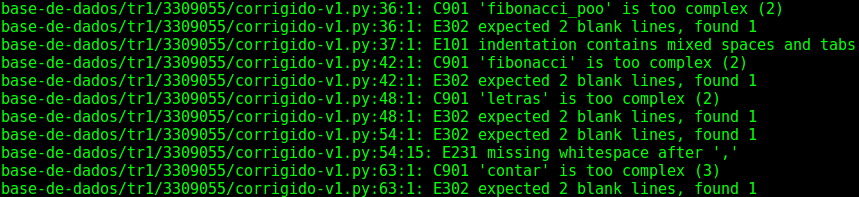
\includegraphics[width=1\linewidth]{imagem/flake8}
				\caption{Representação das características analisadas pelo \texttt{flake8}.}
				\label{fig:flake8}
			\end{figure}		

			A \cref{fig:arquivoCSV} apresenta o arquivo gerado pelas ferramentas após a
			execução das análises de cada código-fonte presente no repositório analisado.
			As três primeiras colunas são: o nome do arquivo, a quantidade de linhas implementadas
			e o total de erros do estilo de escrita PEP 8 \cite{van2001pep}, respectivamente. As
			demais colunas são referentes a cada erro do PEP 8, com a última
			coluna representando a complexidade ciclomática calculada pela ferramenta
			\texttt{mccabe} \cite{mccabe2013}.

			\begin{figure}[h]
				\centering
				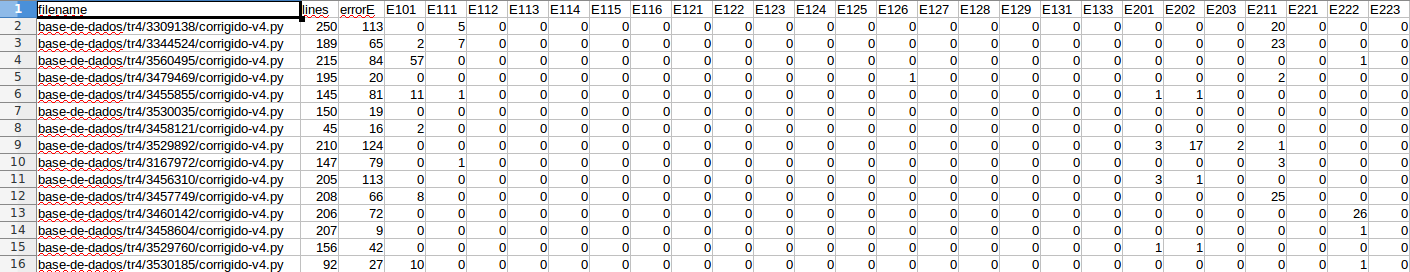
\includegraphics[width=1\linewidth]{imagem/arquivoCSV}
				\caption{Arquivo no formato \texttt{CSV} gerado após as adaptações inseridas nas ferramentas \texttt{flake8} e \texttt{pep8}.}
				\label{fig:arquivoCSV}
			\end{figure}
		

		\subsection{ScienceView}
		\label{sec:scienceView}
		
		A ferramenta \foreign{ScienceView} \cite{Alencar} foi desenvolvida para criar
		mapas de documentos temporais que exibam as mudanças nas as relações entre
		artigos científicos, utilizando a projeção multidimensional dinâmica \acs{T-LSP}
		a partir de artigos nos formatos \foreign{ISI}, \foreign{Endnote Export Format}
		ou \foreign{BibTeX}.
		
		A primeira adaptação na ferramenta condiz com a inserção do novo formato \texttt{CSV}.
		Foi necessário criar um filtro para a extensão \texttt{.csv} a fim que só aparecesse
		os arquivos desse formato no momento de selecionar o arquivo. Em seguida, foi preciso
		realizar a leitura desses dados contidos no arquivo. Assim, foi necessário encontrar
		uma biblioteca disponível no Maven para realizar a leitura do arquivo para obtermos
		as características presentes no cabeçalho, nome do arquivo e a quantidade de cada
		erro desse arquivo para pode inserir no banco de dados da ferramenta. Inserimos novos
		comandos \texttt{SQL} para guardar todas as informações da leitura no banco de dados.
		Toda matriz esparsa obtida na leitura é salva no banco de dados para que seja
		utilizada como base para o cálculo da matriz de similaridade.
		
		Originalmente, a ferramenta suportava apenas números inteiros em sua representação
		interna. No entanto, alguns dos valores importados do formato \texttt{CSV} podem
		ser números reais. Desta forma, foram alteradas as formas de representação e cálculos
		para utilizar números em ponto flutuante de precisão dupla.
		
		Modificamos também a ferramenta para que, ao clicar duas vezes em um marcador visual
		na projeção (que representa um código fonte), seja mostrado o código-fonte referente
		ao marcador (programa sob avaliação) e
		seu vetor de características (com e sem normalização).
		
		A fim de criar uma nova projeção multidimensional dinâmica, a ferramenta guia o
		usuário para: inserir um novo conjunto de dados ou utilizar uma coleção presente
		no banco de dados; definir parâmetros sobre o pré-processamentos dos dados; decidir
		qual cálculo de similaridade será utilizado; e determinar os parâmetros referente
		a \acs{T-LSP}.
	
		\begin{figure}[b]
			\centering
			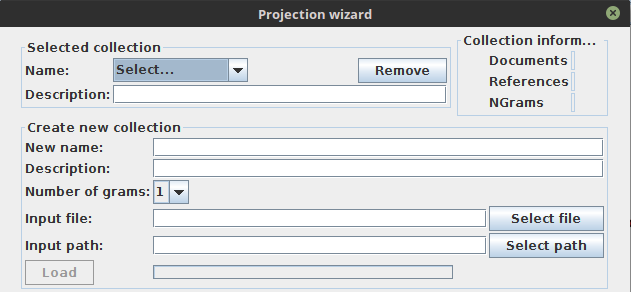
\includegraphics[width=0.8\linewidth]{imagem/createDatabase}
			\caption{Interface para selecionar coleção e inserir nova coleção na base de dados}
			\label{fig:createDatabase}
		\end{figure}
		
		A \cref{fig:createDatabase} apresenta os painéis para selecionar uma coleção existente
		e inserir uma nova coleção na base de dados. Para acrescer uma nova coleção na base,
		clique no botão \foreign{Select file}, altere o filtro do tipo do arquivo, selecionando
		o arquivo \texttt{CSV (*.csv)}. Depois clique no botão \foreign{Select path} e selecione
		o caminho que está as implementações. Esse caminho deve conter a primeira pasta do
		arquivo descrito no arquivo \texttt{CSV}. Clique em \foreign{Load} para inserir a
		coleção na base de dados e selecione a coleção que acabou de ser inserida, clicando
		em \foreign{Select} no painel \foreign{Selected collection}.
		
		A \cref{fig:normalizacao} apresenta o painel para seleção do cálculo de normalização
		descrito como \foreign{Normalization}. É possível selecionar o cálculo que deseja
		utilizar ao clicar em \texttt{NONE}. Será apresentado todos os cálculos de
		normalização disponíveis.
		
		\begin{figure}
			\centering
			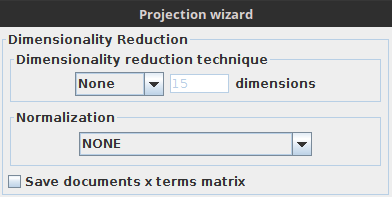
\includegraphics[width=0.5\linewidth]{imagem/normalizacao}
			\caption{Interface para selecionar o cálculo de normalização.}
			\label{fig:normalizacao}
		\end{figure}
		
		A \cref{fig:similaridade} apresenta o painel para escolha do cálculo de similaridade
		descrito como \foreign{Choose the Distance Type}. É possível selecionar o cálculo de
		similaridade que deseja utilizar, clicando em \foreign{Cosine-based}. Então, sera
		apresentado todas os cálculos de similaridade disponíveis na ferramenta.
		
		\begin{figure}
			\centering
			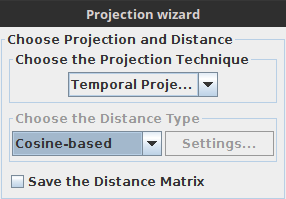
\includegraphics[width=0.35\linewidth]{imagem/similaridade}
			\caption{Interface para selecionar o cálculo de similaridade.}
			\label{fig:similaridade}
		\end{figure}
		
		
		A \cref{fig:projecao} apresenta a interface inicial para verificar a visualização da
		projeção. É possível visualizar o desenvolvimento da projeção de duas formas: clicando no botão
		com o ícone \foreign{Play}; ou visualizar cada projeção na sequência de projeções
		interagindo com a barra de progressão da visualização, localizada na parte inferior
		da interface ao lado dos botões, clicando no botão com o ícone \foreign{Forward}.
		Ao final, dado que a sequência de projeções é cumulativa, será apresentado a projeção
		completa, conforme a \cref{fig:projecaoFinal}, na qual cada ponto corresponde a uma
		implementação e, ao clicar duas vezes, é apresentado seu código-fonte, bem como a
		quantidade de erros e seus valores normalizados.
		
		\begin{figure}
			\centering
			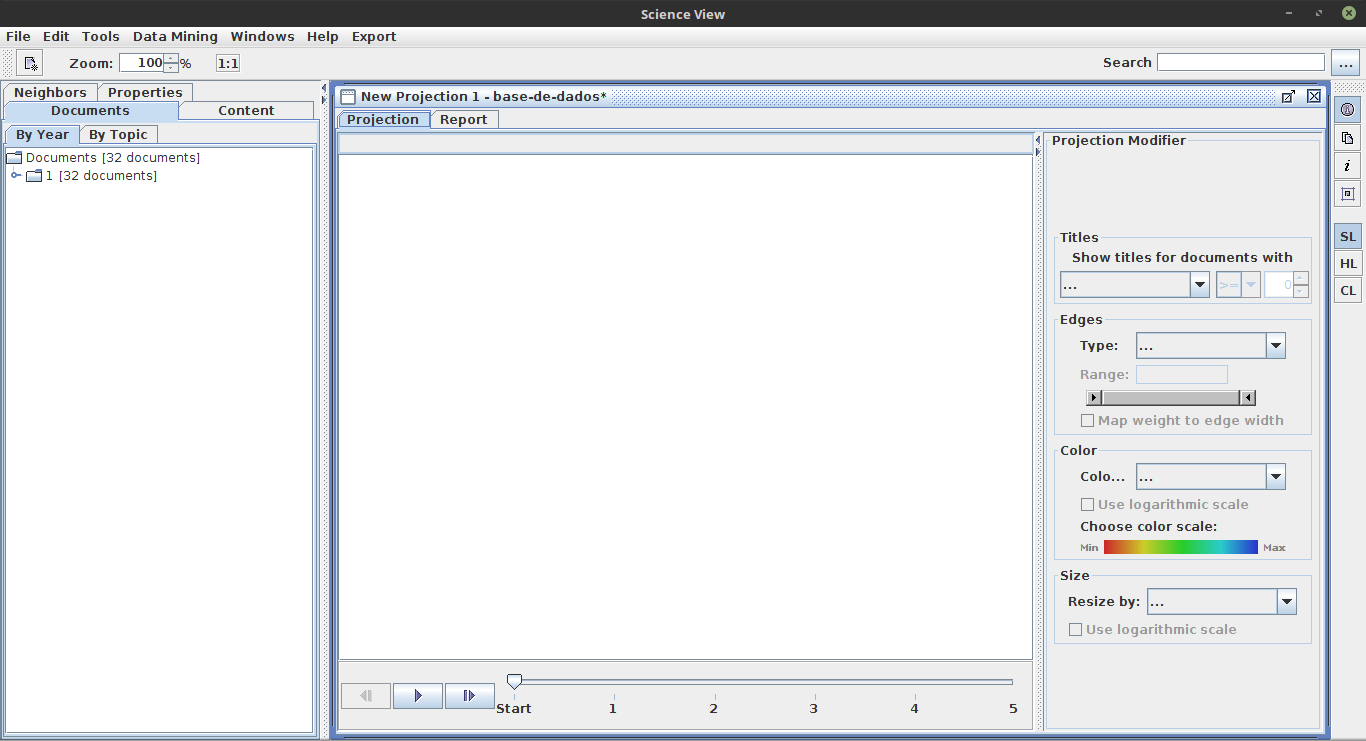
\includegraphics[width=1\linewidth]{imagem/projecao}
			\caption{Interface inicial da visualização.}
			\label{fig:projecao}
		\end{figure}
		
		Também é possível ativar a extração de tópicos ao decorrer das projeções. Desta
		forma é possível visualizar os agrupamentos encontrados pela \foreign{ScienceView},
		bem como os tópicos ou características de cada grupo. A \cref{fig:topics3}
		exibe os agrupamentos formados pela ferramenta no decorrer da projeção no instante
		de tempo $3$. É possível verificar os agrupamentos formados, pois eles são
		visualmente delimitados por polígonos  na cor cinza e, para cada agrupamento,
		são apresentadas as características relevantes àquele agrupamento. A ferramenta
		também realiza o rastreamento dos grupos simultaneamente. Consequentemente, além
		de gerar os grupos para cada projeção na sequência, a \foreign{ScienceView}
		também rastreia esses grupos ao longo do tempo. A extração de tópicos e o
		rastreamento podem ser ativados pelo menu superior, clicando em:
		\foreign{Data Mining}, \foreign{Topic Extraction and Tracking} e \foreign{Run}.
		
		\begin{figure}
			\centering
			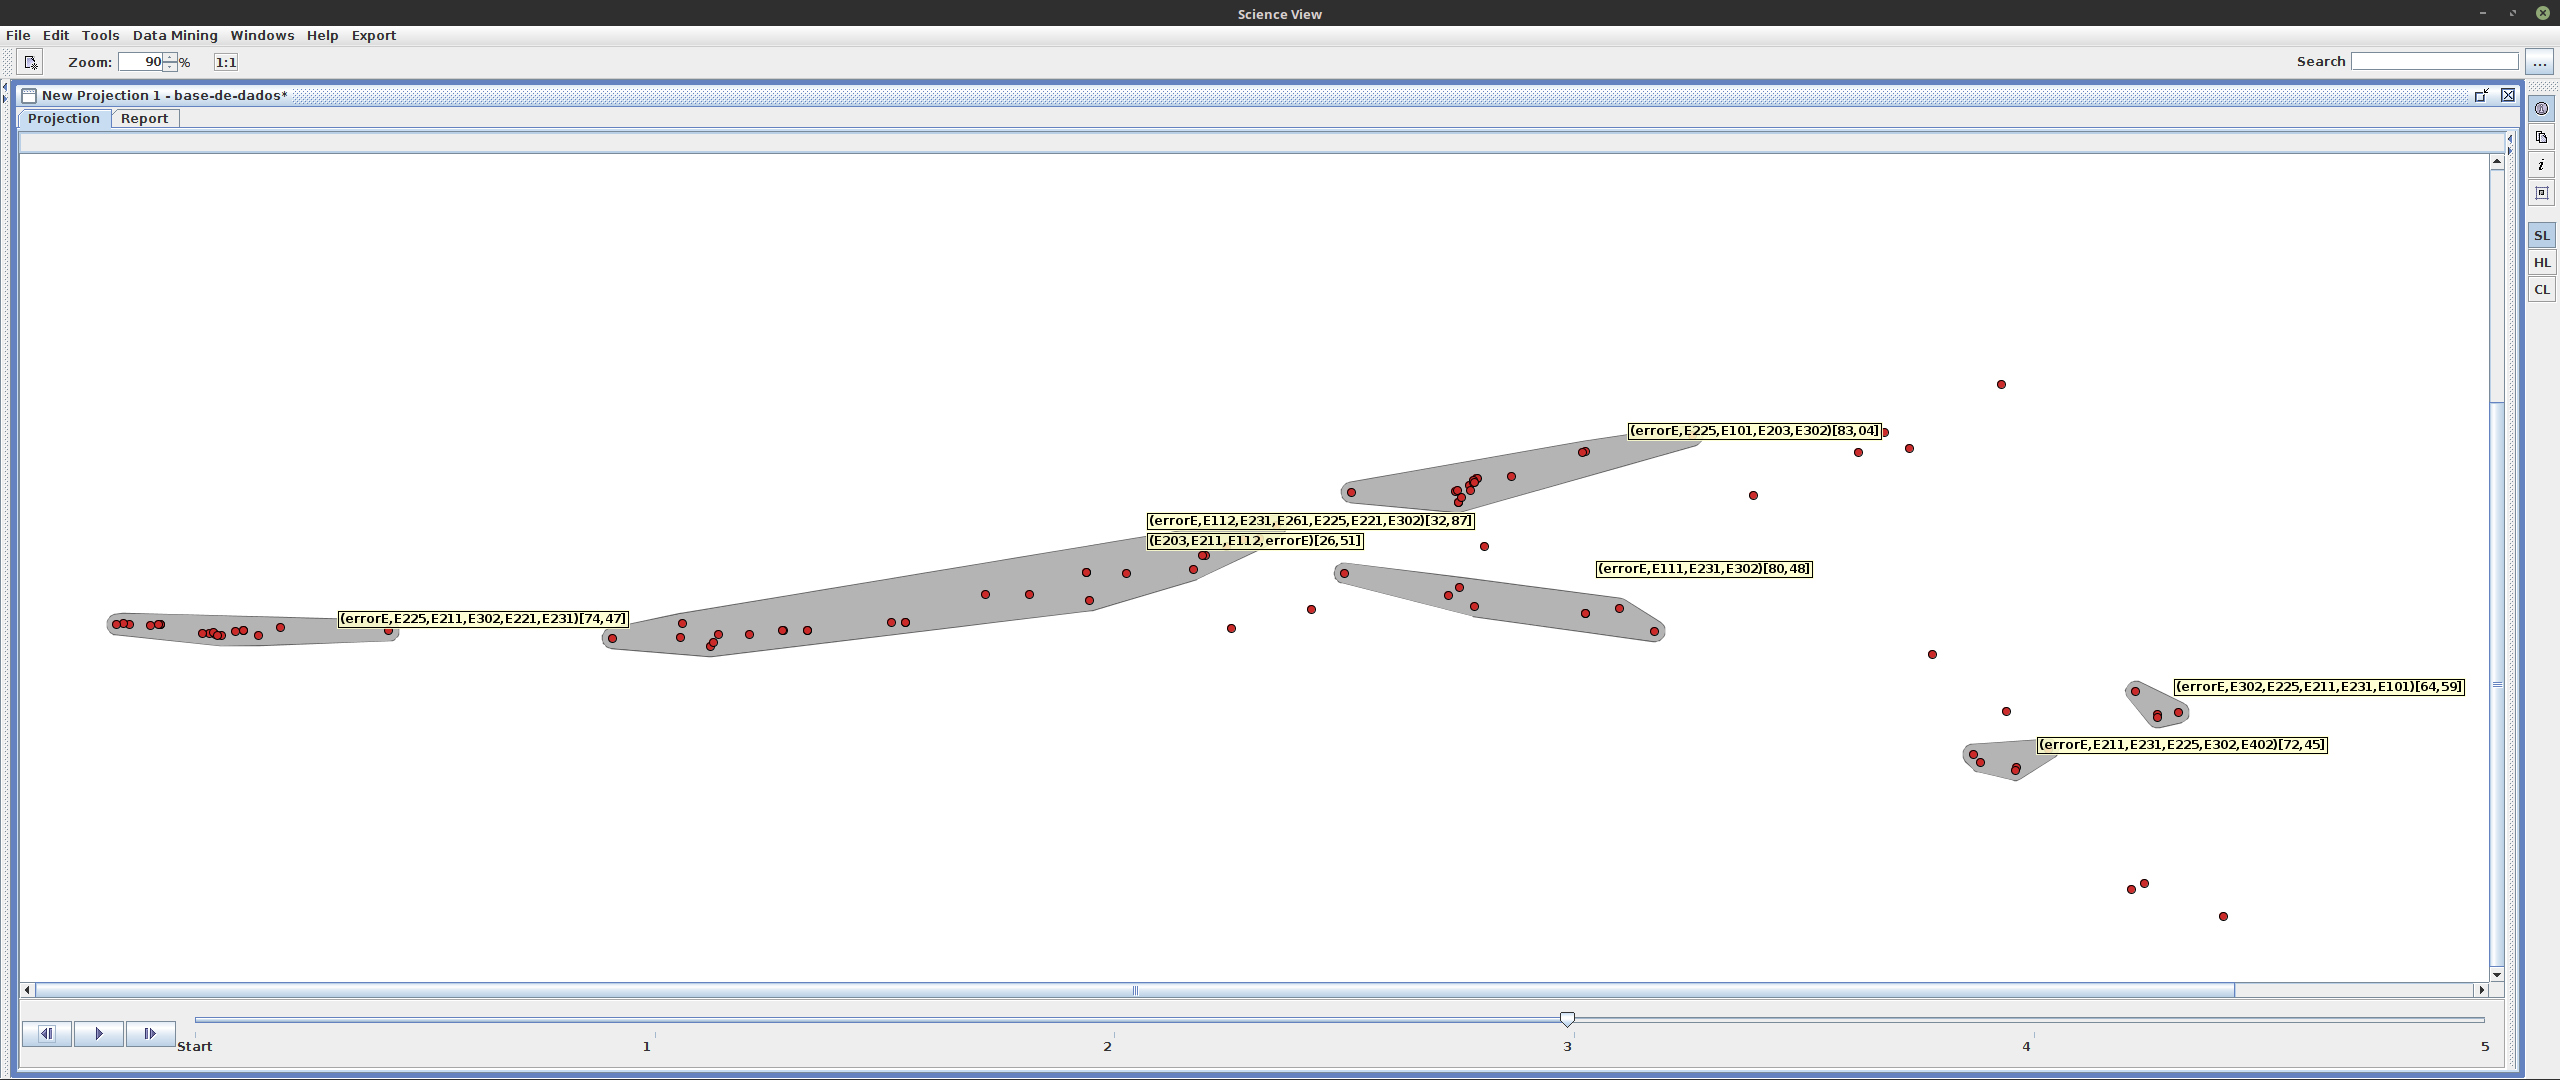
\includegraphics[width=1\linewidth]{imagem/topics3}
			\caption{Final da exibição das projeções com a extração de tópicos ativada.}
			\label{fig:topics3}
		\end{figure}
		
		A \cref{fig:multiplosDoc} exibe a possibilidade de abrir mais de uma implementação
		em uma mesma janela, utilizando abas. Para habilitar esse recurso, é necessário
		clicar no segundo botão no painel vertical a direita. Ao deixa o cursor sobre esse
		botão, aparecerá o seguinte texto: \foreign{View Content}. Em seguida, selecione
		as implementações que deseja abrir, mantendo o botão esquerdo do \foreign{mouse}
		pressionado e enquadrando na área verde, as implementações que deseja abrir na
		mesma janela.
		
		\begin{figure}[t]
			\centering
			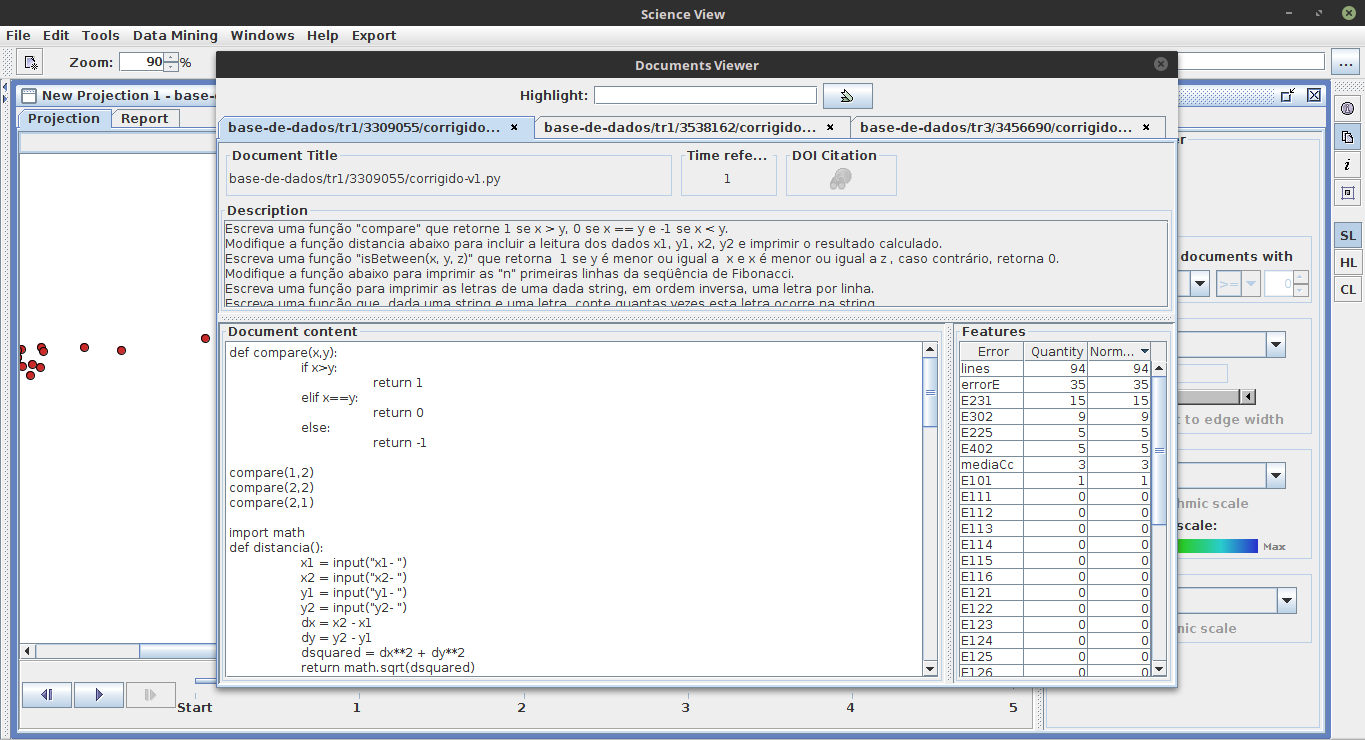
\includegraphics[width=.95\linewidth]{imagem/multiplosDoc}
			\caption{Abrir várias implementações em uma única janela.}
			\label{fig:multiplosDoc}
		\end{figure}
		
		A \cref{fig:ladoAlado} apresenta a possibilidade de abrir uma implementação em
		cada janela para que seja possível comparar a tabela de erros, por exemplo.
		Para abrir cada implementação em uma janela diferente, clique duas vezes com
		o botão esquerdo do \foreign{mouse} sobre o ponto da implementação. O
		visualizador da implementações permite redimensionar sua janela, bem como
		cada painel.
		
		\begin{figure}[hb]
			\centering
			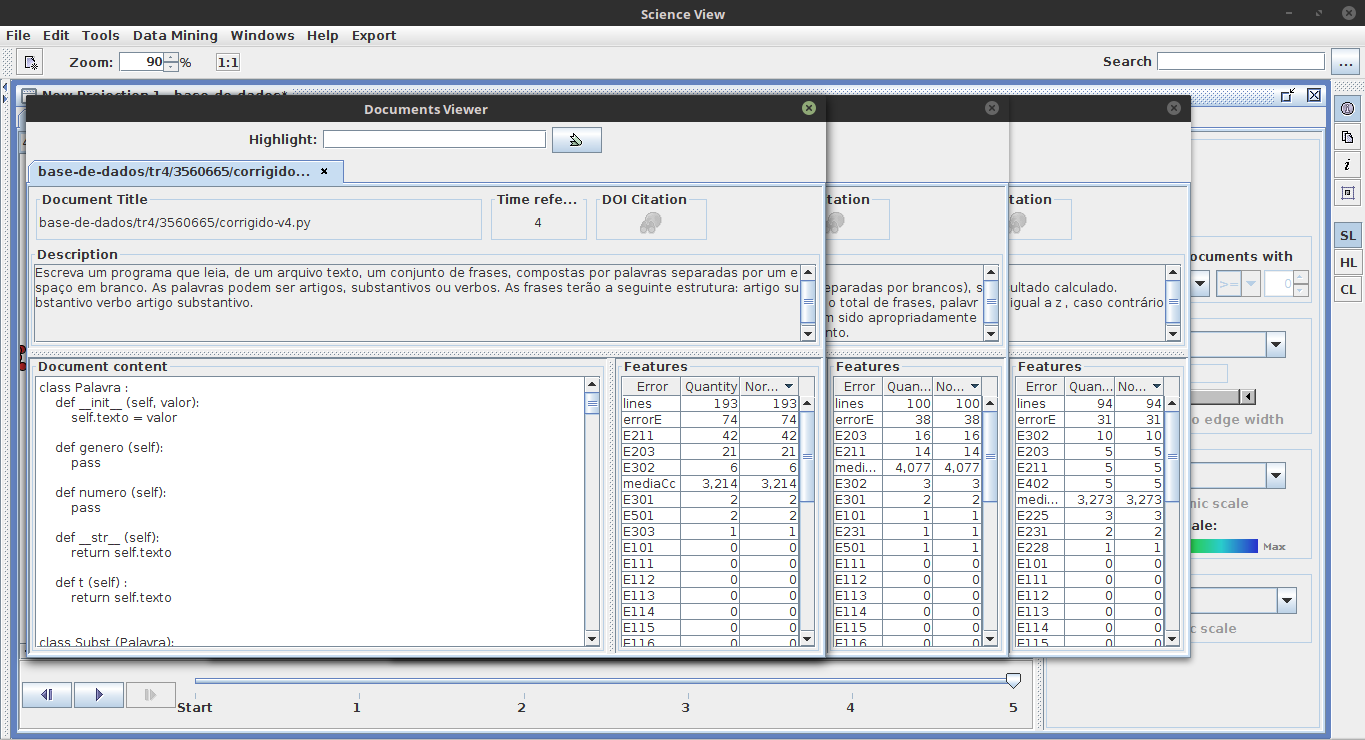
\includegraphics[width=.95\linewidth]{imagem/ladoAlado}
			\caption{Varias implementações abertas em janelas diferentes.}
			\label{fig:ladoAlado}
		\end{figure}
		

	\section{Considerações finais}
	
		Utilizando o método e as ferramentas descritas neste capítulo,
		o próximo capítulo apresenta um estudo sobre avaliação de programas em Python,
		descrevendo a base de dados, a forma que foi realizado
		seu experimento sua avaliação e os resultados.